\documentclass[12pt,a4paper]{article}

% ── Core packages ──────────────────────────────────────────────────
\usepackage[utf8]{inputenc}
\usepackage[T1]{fontenc}
\usepackage{lmodern}             % Crisp modern font
\usepackage{geometry}
\geometry{a4paper, margin=0.85in, top=1in, bottom=1in}
\usepackage{xcolor}
\usepackage{hyperref}
\usepackage{enumitem}
\usepackage{titlesec}
\usepackage{tcolorbox}
\tcbuselibrary{skins, breakable, listingsutf8}
\usepackage{listings}
\usepackage{tikz}
\usetikzlibrary{shapes.geometric, arrows.meta, positioning, shadows}
\usepackage{mdframed}
\usepackage{fontawesome5}
\usepackage{booktabs}
\usepackage{microtype}

% ── Color Palette ──────────────────────────────────────────────────
\definecolor{foldercolor}{RGB}{31, 119, 180}       % Folder blue
\definecolor{filecolor}{RGB}{127, 127, 127}        % File grey
\definecolor{accentcolor}{RGB}{44, 160, 44}        % Green accent

\definecolor{sectioncolor}{RGB}{10, 50, 120}       % Deep navy
\definecolor{subsectioncolor}{RGB}{0, 102, 204}    % Bright blue
\definecolor{subsubsectioncolor}{RGB}{0, 140, 90}  % Teal green
\definecolor{questioncolor}{RGB}{140, 20, 20}      % Dark crimson
\definecolor{answercolor}{RGB}{0, 110, 50}         % Forest green
\definecolor{keywordcolor}{RGB}{180, 90, 0}        % Amber orange

\definecolor{boxblue}{RGB}{220, 235, 255}          % Light blue bg
\definecolor{boxblueborder}{RGB}{0, 80, 180}       % Blue border
\definecolor{boxgreen}{RGB}{220, 245, 230}         % Light green bg
\definecolor{boxgreenborder}{RGB}{0, 120, 60}      % Green border
\definecolor{boxred}{RGB}{255, 230, 225}           % Light red bg
\definecolor{boxredborder}{RGB}{160, 30, 30}       % Red border
\definecolor{boxamber}{RGB}{255, 248, 220}         % Amber bg
\definecolor{boxamberborder}{RGB}{180, 100, 0}     % Amber border
\definecolor{codebg}{RGB}{245, 245, 248}           % Code background
\definecolor{codeframe}{RGB}{190, 190, 210}        % Code frame

% ── Section Formatting ─────────────────────────────────────────────
\titleformat{\section}
  {\normalfont\Large\bfseries\color{sectioncolor}}
  {\thesection}{1em}{}[{\color{sectioncolor}\titlerule[1.5pt]}]

\titleformat{\subsection}
  {\normalfont\large\bfseries\color{subsectioncolor}}
  {\thesubsection}{1em}{}[{\color{subsectioncolor!50}\titlerule[0.6pt]}]

\titleformat{\subsubsection}
  {\normalfont\normalsize\bfseries\color{subsubsectioncolor}}
  {\thesubsubsection}{1em}{}

% ── Listings (Code Blocks) ─────────────────────────────────────────
\lstdefinestyle{jsStyle}{
  language=Java,
  backgroundcolor=\color{codebg},
  basicstyle=\ttfamily\small\color{black},
  keywordstyle=\bfseries\color{blue!70!black},
  stringstyle=\color{green!50!black},
  commentstyle=\itshape\color{gray!70},
  numberstyle=\tiny\color{gray},
  numbers=left,
  numbersep=6pt,
  frame=single,
  rulecolor=\color{codeframe},
  breaklines=true,
  showstringspaces=false,
  tabsize=2,
  captionpos=b,
  xleftmargin=8pt,
}
\lstdefinestyle{cppStyle}{
  language=C++,
  backgroundcolor=\color{codebg},
  basicstyle=\ttfamily\small\color{black},
  keywordstyle=\bfseries\color{purple!80!black},
  stringstyle=\color{green!50!black},
  commentstyle=\itshape\color{gray!70},
  numberstyle=\tiny\color{gray},
  numbers=left,
  numbersep=6pt,
  frame=single,
  rulecolor=\color{codeframe},
  breaklines=true,
  showstringspaces=false,
  tabsize=2,
}
\lstset{style=jsStyle}  % default

% ── tcolorbox Styles ───────────────────────────────────────────────
\tcbset{
  conceptbox/.style={
    enhanced, breakable,
    colback=boxblue, colframe=boxblueborder,
    fonttitle=\bfseries\color{boxblueborder},
    attach boxed title to top left={yshift=-2mm, xshift=4mm},
    boxed title style={colback=boxblueborder, colframe=boxblueborder},
    boxrule=0.8pt, arc=4pt,
    left=6pt, right=6pt, top=8pt, bottom=6pt,
  },
  answerbox/.style={
    enhanced, breakable,
    colback=boxgreen, colframe=boxgreenborder,
    fonttitle=\bfseries\color{boxgreenborder},
    boxrule=0.8pt, arc=4pt,
    left=6pt, right=6pt, top=4pt, bottom=4pt,
  },
  warningbox/.style={
    enhanced, breakable,
    colback=boxred, colframe=boxredborder,
    fonttitle=\bfseries\color{boxredborder},
    boxrule=0.8pt, arc=4pt,
    left=6pt, right=6pt, top=4pt, bottom=4pt,
  },
  keybox/.style={
    enhanced, breakable,
    colback=boxamber, colframe=boxamberborder,
    fonttitle=\bfseries\color{boxamberborder},
    boxrule=0.8pt, arc=4pt,
    left=6pt, right=6pt, top=4pt, bottom=4pt,
  },
}

% ── Helper macros ──────────────────────────────────────────────────
\newcommand{\keyword}[1]{\textcolor{keywordcolor}{\textbf{#1}}}
\newcommand{\Q}[1]{\textcolor{questioncolor}{\textbf{#1}}}
\newcommand{\A}{\textcolor{answercolor}{\textbf{Answer:}}}
\newcommand{\codeinline}[1]{\texttt{\small #1}}

\begin{document}

\section*{Project File Structure \& Organization}

The IoT Virtual Laboratory project is organized into a modular 4-tier architecture. This ensures clear separation of concerns between hardware firmware, cloud processing, user interface, and documentation. Below is the comprehensive directory structure and an explanation of the core components.
\vspace{0.4cm}
\begin{center}
\begin{tcolorbox}[conceptbox, title=\faProjectDiagram\; System Architecture Overview]
\resizebox{\linewidth}{!}{
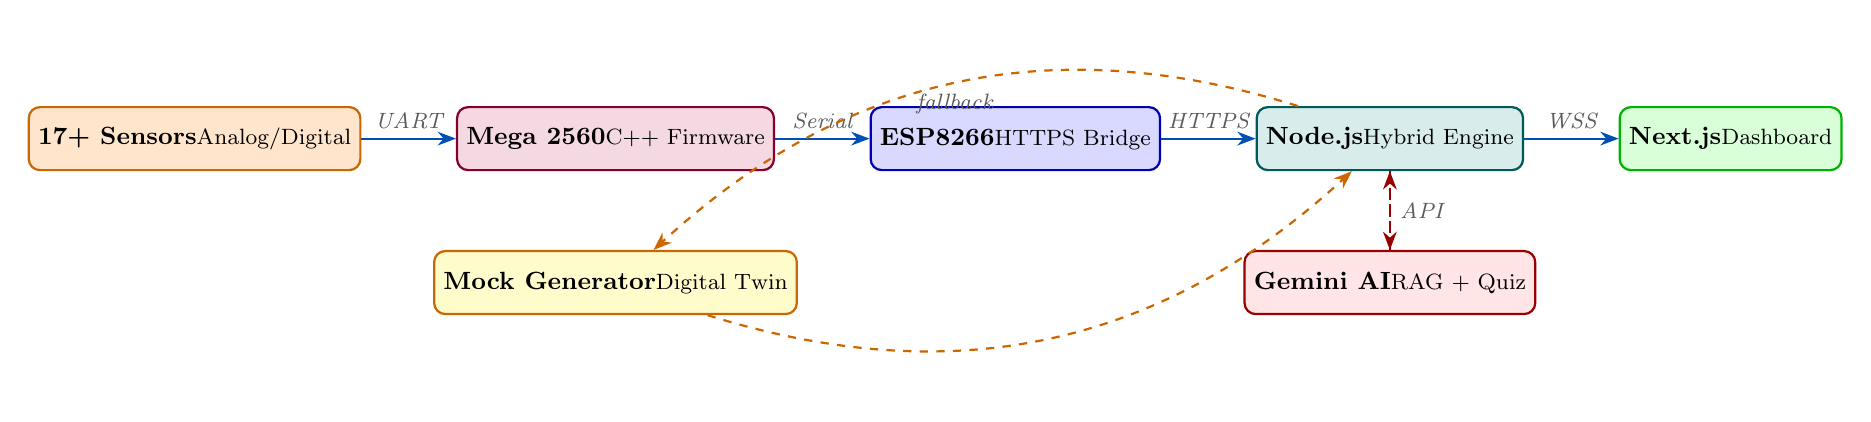
\begin{tikzpicture}[
  node distance=0.7cm and 1.2cm,
  every node/.style={font=\small},
  box/.style={rectangle, rounded corners=4pt, draw, thick, minimum width=2.5cm, minimum height=0.8cm, text centered, fill=boxblue, draw=boxblueborder},
  arrow/.style={-Stealth, thick, color=boxblueborder},
  label/.style={font=\footnotesize\itshape, color=gray!70!black},
]
  \node[box, fill=orange!20, draw=orange!80!black] (sensors) {\textbf{17+ Sensors}\\\footnotesize Analog/Digital};
  \node[box, fill=purple!15, draw=purple!70!black, right=of sensors] (mega) {\textbf{Mega 2560}\\\footnotesize C++ Firmware};
  \node[box, fill=blue!15, draw=blue!70!black, right=of mega] (esp) {\textbf{ESP8266}\\\footnotesize HTTPS Bridge};
  \node[box, fill=teal!15, draw=teal!70!black, right=of esp] (nodejs) {\textbf{Node.js}\\\footnotesize Hybrid Engine};
  \node[box, fill=green!15, draw=green!70!black, right=of nodejs] (frontend) {\textbf{Next.js}\\\footnotesize Dashboard};

  \draw[arrow] (sensors) -- node[above, label]{UART} (mega);
  \draw[arrow] (mega) -- node[above, label]{Serial} (esp);
  \draw[arrow] (esp) -- node[above, label]{HTTPS} (nodejs);
  \draw[arrow] (nodejs) -- node[above, label]{WSS} (frontend);

  \node[box, fill=red!10, draw=red!60!black, below=1.0cm of nodejs] (gemini) {\textbf{Gemini AI}\\\footnotesize RAG + Quiz};
  \draw[arrow, dashed, color=red!60!black] (nodejs) -- node[right, label]{API} (gemini);
  \draw[arrow, dashed, color=red!60!black] (gemini) -- (nodejs);

  \node[box, fill=yellow!20, draw=orange!80!black, below=1.0cm of mega] (mock) {\textbf{Mock Generator}\\\footnotesize Digital Twin};
  \draw[arrow, dashed, color=orange!80!black] (nodejs) to[bend right=30] node[below, label]{fallback} (mock);
  \draw[arrow, dashed, color=orange!80!black] (mock) to[bend right=30] (nodejs);
\end{tikzpicture}
}
\end{tcolorbox}
\end{center}
\vspace{0.3cm}


\vspace{0.5cm}

\subsection*{Directory Tree}

\begin{itemize}[label=\textcolor{foldercolor}{\textbf{/}}]
    \item \textbf{\textcolor{foldercolor}{backend/}} : Node.js Server and API Gateway
    \begin{itemize}[label=--]
        \item \textcolor{filecolor}{\codeinline{server.js}} : The core Express/Socket.io server handling hardware data, AI integration (Gemini), and real-time client streaming.
        \item \textcolor{filecolor}{\codeinline{mockDataGenerator.js}} : Mathematical models (sine waves) simulating sensor behavior when hardware is disconnected (\keyword{Digital Twin} fallback).
        \item \textcolor{filecolor}{\codeinline{package.json}} : Backend dependencies.
    \end{itemize}

    \item \textbf{\textcolor{foldercolor}{firmware/}} : Hardware Code (C++)
    \begin{itemize}[label=--]
        \item \textbf{\textcolor{foldercolor}{Mega2560\_Main/}} : Data Acquisition Layer
        \begin{itemize}[label=-]
            \item \textcolor{filecolor}{\codeinline{Mega2560\_Main.ino}} : Polls 17+ analog/digital sensors and serializes data into a single JSON payload.
        \end{itemize}
        \item \textbf{\textcolor{foldercolor}{esp8266\_bridge/}} : Network Communication Layer
        \begin{itemize}[label=-]
            \item \textcolor{filecolor}{\codeinline{esp8266\_bridge.ino}} : Receives UART serial data from the Mega and pushes HTTP POST requests to the backend server.
        \end{itemize}
    \end{itemize}

    \item \textbf{\textcolor{foldercolor}{frontend/}} : Presentation Layer (Next.js/React)
    \begin{itemize}[label=--]
        \item \textbf{\textcolor{foldercolor}{src/app/}} : Main application routes.
        \begin{itemize}[label=-]
            \item \textbf{\textcolor{foldercolor}{sensors/}} : Individual dynamic routes for each sensor's detailed dashboard.
            \item \textbf{\textcolor{foldercolor}{experiments/}} : Interactive virtual laboratory sessions.
        \end{itemize}
        \item \textbf{\textcolor{foldercolor}{src/components/}} : Reusable React UI components (Gauges, Charts, AI Chatbox).
        \item \textbf{\textcolor{foldercolor}{src/config/}} : 
        \begin{itemize}[label=-]
            \item \textcolor{filecolor}{\codeinline{sensorGroups.ts}} : Centralized configuration defining sensor constraints, limits, and visual grouping.
        \end{itemize}
    \end{itemize}

    \item \textbf{\textcolor{foldercolor}{showcase/}} : Presentation and Media
    \begin{itemize}[label=--]
        \item \textbf{\textcolor{foldercolor}{src/app/ppt/}} : Interactive, web-based presentation slides (Next.js) used for project defense.
    \end{itemize}

    \item \textbf{\textcolor{foldercolor}{documentation/}} : Project Literature
    \begin{itemize}[label=--]
        \item \textbf{\textcolor{foldercolor}{sensors/}} : Markdown files for each sensor used as \keyword{RAG} (\keyword{Retrieval-Augmented Generation}) context for the Gemini AI.
        \item \textcolor{filecolor}{\codeinline{SYSTEM\_ARCHITECTURE.md}} : High-level overview of the M.C.N.P logic.
    \end{itemize}

    \item \textcolor{filecolor}{\codeinline{start-local.bat}} : Windows batch script to launch both frontend and backend concurrently for local testing.
\end{itemize}

\vspace{0.5cm}

\subsection*{Architectural Highlights}

\begin{tcolorbox}[keybox, title=\faStar\; Three Pillars of the System]
\begin{enumerate}
    \item \Q{Hybrid Logic Engine (\codeinline{backend/server.js})}: The backend dynamically merges physical hardware data with simulated digital twin data. If a physical sensor disconnects, the system falls back to mathematical simulation within 30 seconds.
    \item \Q{Real-Time Streaming}: Data is pushed from the server to the client using \keyword{WebSockets} (Socket.io) at 5Hz (200ms latency), completely bypassing standard HTTP polling delays.
    \item \Q{Contextual AI}: The \codeinline{documentation/sensors/} directory isn't just for reading; it acts as the knowledge base for the Gemini AI, preventing hallucinations when answering student questions or generating quizzes.
\end{enumerate}
\end{tcolorbox}

\vspace{0.5cm}

\subsection*{Code Explanation: \codeinline{backend/server.jsjs}}

The \texttt{server.js} file is the central nervous system of the IoT Virtual Laboratory. It handles real-time data ingestion, mock data generation, and AI inference.

\begin{itemize}
    \item \Q{Hybrid Merge Logic (\codeinline{mergeHardwareWithMock})}:
    This is the core of the \keyword{Digital Twin} feature. The server dynamically merges live hardware readings into the mathematically generated mock data payload.
\begin{verbatim}
const mergeHardwareWithMock = (mock, real) => {
  if (!real) return mock;
  const merged = JSON.parse(JSON.stringify(mock));
  REAL_SENSORS.forEach(sensorKey => {
    if (real[sensorKey]) {
      merged.sensors[sensorKey] = { 
        ...merged.sensors[sensorKey], 
        ...real[sensorKey],
        isReal: true // Flags data as coming from physical hardware
      };
    }
  });
  return merged;
};
\end{verbatim}

    \item \Q{Hardware Failover (Stale Data Timeout)}:
    A robust fault-tolerance mechanism. If the ESP8266 stops transmitting for 30 seconds, the server automatically discards the stale hardware state and falls back entirely to the mock data stream, preventing frozen dashboards.
\begin{verbatim}
let lastRealDataTime = 0;
const REAL_DATA_TIMEOUT = 30000; // 30 seconds

// Inside the 200ms setInterval loop:
if (useRealData && (Date.now() - lastRealDataTime > REAL_DATA_TIMEOUT)) {
  console.log('[HYBRID] Real data stale (30s). Reverting to mock data.');
  useRealData = false; 
  lastHardwareSensors = null;
}
\end{verbatim}

    \item \Q{Contextual AI Chat Endpoint}:
    Constructs a \keyword{RAG} (\keyword{Retrieval-Augmented Generation}) prompt for Gemini by injecting live sensor data directly into the system prompt.
\begin{verbatim}
app.post("/api/ai-chat", async (req, res) => {
  const { message, context, history } = req.body || {};
  const systemPrompt = `You are an expert IoT Virtual Lab Assistant. 
  The student is currently viewing: ${context?.sensor}.
  Live Data Snippet: ${JSON.stringify(context?.dataSnippet)}.`;
  
  // Model generation logic...
});
\end{verbatim}

    \item \Q{AI Quiz Generator (JSON Mode Enforcement)}:
    Reads markdown documentation dynamically and forces the Gemini API to return a strictly formatted JSON array using \texttt{responseMimeType}.
\begin{verbatim}
app.post("/api/ai-quiz", async (req, res) => {
  // ... reads documentation ...
  const result = await model.generateContent({
      contents: [{ role: "user", parts: [{ text: prompt }] }],
      generationConfig: {
          responseMimeType: "application/json" // Guarantees parseable output
      }
  });
  // ... sends JSON to frontend ...
});
\end{verbatim}

    \item \Q{The Data Streaming Engine}:
    A non-blocking interval that syncs backend emission with the hardware push rate (5Hz) to maintain sub-200ms end-to-end latency.
\begin{verbatim}
// Runs at 200ms (5Hz) to match firmware TX_INTERVAL
setInterval(() => {
  // Always generate mock data
  const mock = generateMockData();
  
  // Merge real data if available and not stale
  latestReading = mergeHardwareWithMock(mock, lastHardwareSensors);
  
  // Stream to all connected clients instantly
  io.emit('data_stream', latestReading);
}, 200); 
\end{verbatim}
\end{itemize}

\vspace{0.5cm}

\subsection*{Code Explanation: \codeinline{backend/mockDataGenerator.js}s}

This file generates continuous, mathematically simulated data for all sensors, serving as the "\keyword{Digital Twin}" base layer when physical hardware is disconnected. It uses sine waves to create realistic data oscillations rather than pure random noise.

\begin{itemize}
    \item \Q{Sine Wave Data Generation}:
\begin{verbatim}
const generateMockData = () => {
    const time = Date.now() / 1000;
    return {
        sensors: {
            dht11: {
                temp: parseFloat((24 + Math.sin(time * 0.1) * 2).toFixed(1)),
                humidity: parseFloat((60 + Math.sin(time * 0.1) * 10).toFixed(1)),
                isReal: false
            },
            // Generates similar oscillating values for 17+ sensors
        }
    };
};
\end{verbatim}
\end{itemize}

\vspace{0.5cm}

\subsection*{Code Explanation: \codeinline{backend/package.jsjs}n}

The \texttt{package.json} file defines the necessary dependencies required to run the Node.js backend. The key libraries enable the Express server, \keyword{WebSocket}s, and the Google Gemini AI integration.

\begin{verbatim}
"dependencies": {
  "@google/generative-ai": "^0.24.1", // Google Gemini AI SDK
  "cors": "^2.8.5",                   // Cross-Origin Resource Sharing
  "dotenv": "^17.2.3",                // Environment variable management
  "express": "^5.2.1",                // Web framework
  "socket.io": "^4.8.3"               // Real-time bi-directional streaming
}
\end{verbatim}

\vspace{0.5cm}

\subsection*{Code Explanation: Firmware (\texttt{firmware/})}

The firmware is split across two microcontrollers to separate the real-time sensor polling from the blocking network operations. This dual-core architecture prevents latency spikes.

\subsubsection*{\codeinline{Mega2560\_Main/Mega2560\_Main.ino}}
This is the "Data Acquisition Layer". It uses non-blocking \texttt{millis()} timers to concurrently poll 17 sensors at different frequencies.

\begin{itemize}
    \item \Q{Non-Blocking Multi-Frequency Polling}:
    Instead of using \texttt{delay()}, the Mega uses \texttt{millis()} intervals to poll sensors at optimal rates (Fast: 50ms, Medium: 200ms, DHT: 2000ms). Transient digital inputs (like touch and sound) are logically OR-latched (\texttt{|=}) so micro-triggers are never missed between transmissions.
\begin{verbatim}
if (currentMillis - lastFastUpdate >= INTERVAL_FAST) {
  lastFastUpdate = currentMillis;
  // Latch transient inputs to guarantee they are caught
  sysData.touch_active |= (digitalRead(PIN_TOUCH) == HIGH);
  sysData.sound_d |= (digitalRead(PIN_SOUND_D) == HIGH);
}
\end{verbatim}

    \item \Q{Hardware Handshake Protocol}:
    The Mega waits for an "ACK" from the ESP8266 before sending the next packet. If the ACK is missed due to a UART glitch, a 2000ms timeout forces a recovery transmission.
\begin{verbatim}
// Only send if not waiting for ACK, or TX_TIMEOUT hit
if (!waitingForAck || (currentMillis - lastTXAttempt >= TX_TIMEOUT)) {
  lastTXUpdateRecord = currentMillis;
  lastTXAttempt = currentMillis;
  transmitData(); // Serializes JSON and sends via UART
}
\end{verbatim}

    \item \Q{Precision Math \& Loop Safety (\keyword{Steinhart-Hart} \& Ultrasonic)}:
    Advanced sensor calculations are executed locally on the edge node to reduce backend payload. The Thermistor uses the complex \keyword{Steinhart-Hart} equation with logarithmic approximations to convert raw ADC values to precise Celsius. The Ultrasonic sensor uses a strictly timed \texttt{pulseIn} with a 10,000$\mu s$ timeout to prevent the entire system from freezing if a sound wave echo is lost to the environment.
\begin{verbatim}
// Steinhart-Hart Thermistor approximation
float R_therm = (10000.0 * Vout) / (5.0 - Vout);
float logR = log(R_therm);
float tempK = 1.0 / (0.001129 + (0.000234 * logR) + (0.0000000876 * logR * logR * logR));

// Ultrasonic 10ms safety timeout
long duration = pulseIn(PIN_ECHO, HIGH, 10000); 
sysData.sonic_dist = (duration > 0) ? (duration * 0.0343) / 2.0 : 0.0;
\end{verbatim}
    \item \Q{JSON Serialization \& Memory Efficiency}:
    Instead of concatenating massive strings manually (which rapidly fragments RAM on AVR microcontrollers), the Mega uses the \texttt{ArduinoJson} library. It constructs a \texttt{JsonDocument} and serializes it \textit{directly} to the Serial port stream.
\begin{verbatim}
JsonDocument doc;
doc["device_id"] = "mega_node_01";
JsonObject s = doc["sensors"].to<JsonObject>();
s["dht11"]["temp"] = sysData.ext_temp;
// ... (other sensors) ...
serializeJson(doc, Serial); // Streams bytes directly, no intermediate String buffer!
\end{verbatim}

    \item \Q{Heart Rate / BPM Algorithm}:
    For the MAX30102 medical sensor, the Mega measures the inter-beat interval between detected pulses to calculate real-time BPM, applying a sanity check (30-300 BPM) and a decay timer to reset if the finger is removed.
\begin{verbatim}
if (checkForBeat(sysData.max_ir) == true) {
  unsigned long delta = now - lastBeatTime;
  if (delta > 200 && delta < 2000) { // Sanity: 30-300 BPM range
    sysData.bpm = 60000.0 / (float)delta;
  }
}
\end{verbatim}
\end{itemize}

\subsubsection*{\codeinline{esp8266\_bridge/esp8266\_bridge.ino}}
This is the "Network Communication Layer". It receives the JSON payload via UART and pushes it to the Node.js backend using HTTP POST.

\begin{itemize}
    \item \Q{TLS Session Caching}:
    To achieve low latency (~150ms) over secure HTTPS without the deadlocks caused by TCP Keep-Alive on the ESP8266, the bridge caches the TLS Cryptographic Session. This bypasses the slow SSL handshake on every push.
\begin{verbatim}
BearSSL::Session tlsSession; // Cache TLS keys

void sendToServer(const char* jsonData) {
  // ...
  wifiClient.setSession(&tlsSession); // Resume previous session (FAST!)
  http.begin(wifiClient, SERVER_URL);
  int code = http.POST(payload);
  
  // ALWAYS gracefully close to prevent socket exhaustion
  http.end();
  wifiClient.stop(); 
}
\end{verbatim}

    \item \Q{Memory-Safe Serial Buffer \& Backpressure}:
    Instead of using blocking \texttt{readString()} which fragments heap memory, characters are parsed byte-by-byte into a static buffer. Once parsed, it sends the "ACK" back to the Mega.
\begin{verbatim}
while (Serial.available()) {
  char c = Serial.read();
  if (c == '\n') {
    jsonBuffer[bufferIndex] = '\0'; // Null-terminate
    if (millis() - lastHTTPRequest >= HTTP_INTERVAL) {
      sendToServer(jsonBuffer); // Push to cloud
    }
    Serial.println("ACK"); // Release Mega's transmission lock
    bufferIndex = 0;
  } else if (c != '\r' && bufferIndex < 2047) {
    jsonBuffer[bufferIndex++] = c;
  }
}
\end{verbatim}
    \item \Q{Payload Augmentation \& Diagnostics}:
    Before forwarding the payload to the Cloud, the ESP8266 deserializes the Mega's JSON and injects its own network health metrics. This allows the dashboard to monitor the bridge's physical status.
\begin{verbatim}
DynamicJsonDocument doc(2048);
deserializeJson(doc, jsonData);

JsonObject sys = doc.createNestedObject("system");
sys["rssi"] = WiFi.RSSI();         // Wi-Fi Signal Strength
sys["heap"] = ESP.getFreeHeap();   // Available RAM
sys["uptime_ms"] = millis();       // Stability tracker
\end{verbatim}

    \item \Q{WiFi Watchdog Timer}:
    A non-blocking background task that checks the network connection every 15 seconds. If the router drops the connection, it automatically triggers a reconnection without resetting the hardware.
\begin{verbatim}
if (millis() - lastWifiCheck > 15000) {
  lastWifiCheck = millis();
  if (WiFi.status() != WL_CONNECTED) {
    WiFi.begin(WIFI_SSID, WIFI_PASSWORD); // Auto-recover connection
  }
}
\end{verbatim}
\end{itemize}

\vspace{0.5cm}

\subsection*{Code Explanation: Frontend (\texttt{frontend/src/})}

The frontend is built using Next.js (App Router), React, and Tailwind CSS. It focuses on rendering real-time data efficiently and providing an interactive educational interface.

\subsubsection*{\codeinline{config/sensorGroups.ts}}
This file acts as the "\keyword{Single Source of Truth}" for the entire application. It defines the properties, safety thresholds, and visual metadata (icons, colors) for all 17+ sensors.
\begin{itemize}
    \item \Q{Centralized Configuration}:
    By centralizing metadata, the UI dynamically generates itself based on this configuration, eliminating hardcoded UI elements and ensuring consistency across the dashboard.
\begin{verbatim}
export const SENSOR_GROUPS = [
  {
    id: "environment",
    title: "Environmental Conditions",
    sensors: [
      {
        id: "dht11",
        name: "DHT11 Temp & Humidity",
        metrics: [
          { key: "temp", label: "Temperature", unit: "°C", warning: 30, critical: 40 }
        ]
      }
    ]
  }
];
\end{verbatim}
\end{itemize}

\subsubsection*{\codeinline{hooks/useSocket.ts}}
This custom React hook manages the \keyword{WebSocket} connection lifecycle to the Node.js backend.
\begin{itemize}
    \item \Q{Global Connection Management}:
    It establishes a singleton connection upon component mount and listens for the 5Hz \texttt{data\_stream} events, gracefully disconnecting on unmount to prevent memory leaks.
\begin{verbatim}
useEffect(() => {
    const socketInstance = io(SOCKET_URL);
    
    socketInstance.on("data_stream", (newData: SensorData) => {
        setData(newData); // Triggers React state updates at 5Hz
    });

    return () => socketInstance.disconnect(); // Cleanup on unmount
}, []);
\end{verbatim}
\end{itemize}

\subsubsection*{\codeinline{hooks/useSignalProcessing.ts}}
This hook implements client-side Digital Signal Processing (\keyword{DSP}) to smooth out hardware noise for educational visualization.
\begin{itemize}
    \item \Q{Dynamic Filtering}:
    It provides a \texttt{useMemo} optimized Moving Average filter and Noise Threshold gate, allowing students to toggle \keyword{DSP} algorithms on live data and instantly see the results on their charts.
\begin{verbatim}
const processedData = useMemo(() => {
    switch (filter.type) {
        case 'moving-average': {
            const subset = arr.slice(idx - windowSize + 1, idx + 1);
            return subset.reduce((a, b) => a + b, 0) / subset.length;
        }
        case 'threshold': {
            const diff = Math.abs(val - arr[idx - 1]);
            return diff < filter.threshold ? arr[idx - 1] : val; // Debounce
        }
    }
}, [dataStream, filter]);
\end{verbatim}
\end{itemize}

\subsubsection*{\codeinline{app/sensors/[id]/page.tsx} \& \codeinline{components/Dashboard.tsx}}
The UI layer leverages Next.js dynamic routing and reusable React components.
\begin{itemize}
    \item \Q{Dynamic Rendering \& Real-Time Charts}:
    The \texttt{Dashboard.tsx} maps over \texttt{SENSOR\_GROUPS} to render overview cards, while the dynamic \texttt{[id]} route renders deep-dive analytics for specific sensors, feeding the \texttt{useSocket} data directly into Recharts graphing libraries for high-performance visual feedback.
\end{itemize}

\vspace{0.5cm}

\subsection*{Code Explanation: Showcase \& Documentation}

While the Backend, Firmware, and Frontend form the functional core of the project, the Showcase and Documentation directories ensure the project is presentation-ready and AI-compatible.

\subsubsection*{\codeinline{showcase/src/app/ppt/}}
Instead of using static PowerPoint or PDF slides, the presentation layer is a fully interactive Next.js web application.
\begin{itemize}
    \item \Q{Interactive Defense}: By building the presentation slides as a web app, it allows for live demonstration components, dynamic animations, and perfect styling consistency with the main dashboard.
\end{itemize}

\subsubsection*{\codeinline{documentation/sensors/}}
This directory serves a dual purpose: human readability and machine readability.
\begin{itemize}
    \item \Q{RAG Knowledge Base}: The Markdown files detailing each sensor (e.g., \texttt{dht11.md}) are not just static text. They are dynamically ingested by the Node.js backend to provide context to the Gemini AI. This ensures the AI provides accurate, curriculum-specific answers and generates relevant quizzes based strictly on the provided syllabus, preventing AI hallucinations.
\end{itemize}

\vspace{0.5cm}

\subsection*{Code Explanation: Security \& Deployment}

\subsubsection*{Environment Variables (\codeinline{backend/.env})}
To ensure security and prevent secret-leakage to public repositories like GitHub, all sensitive configuration is decoupled from the codebase using a \texttt{.env} file.
\begin{itemize}
    \item \Q{API Key Protection}: The \texttt{GEMINI\_API\_KEY} is stored here securely and loaded into the Node.js runtime via the \texttt{dotenv} library.
    \item \Q{CORS Configuration}: The \texttt{CORS\_ORIGIN} variable defines which frontend domains are permitted to communicate with the backend via \keyword{WebSocket}s/HTTP, preventing Cross-Origin vulnerabilities.
\end{itemize}

\subsubsection*{Local Deployment (\codeinline{start-local.bat})}
A custom Windows batch script engineered to streamline the developer experience and project presentation.
\begin{itemize}
    \item \Q{Concurrent Orchestration}: The script automatically checks for the \texttt{node} runtime, installs missing \texttt{node\_modules} on the fly if needed, and concurrently boots both the Next.js frontend and Node.js backend in parallel terminal windows, eliminating manual startup friction during demonstrations.
\end{itemize}

\vspace{0.5cm}


\vspace{0.5cm}
\begin{tcolorbox}[conceptbox, title=\faTable\; Quick-Reference: Tech Stack \& Responsibilities]
\renewcommand{\arraystretch}{1.3}
\begin{tabular}{p{2.8cm} p{3.0cm} p{5.5cm}}
  \toprule
  \textbf{Layer} & \textbf{Technology} & \textbf{Key Responsibility} \\
  \midrule
  Sensor Polling  & Arduino Mega 2560 (C++) & Non-blocking 17+ sensor acquisition at multi-Hz rates \\
  Network Bridge  & ESP8266 (C++)           & TLS-secured HTTPS POST with ACK handshake \\
  Backend Engine  & Node.js / Express       & Digital Twin hybrid merge + AI API gateway \\
  Real-Time Comm. & Socket.io (WebSockets)  & Sub-200ms push streaming at 5Hz \\
  AI Integration  & Google Gemini 2.5 Flash & RAG-grounded chat, quiz, and graph analysis \\
  Frontend UI     & Next.js / React         & Dynamic sensor dashboard + client-side DSP \\
  Documentation   & Markdown (.md)          & RAG knowledge base for Gemini context \\
  \bottomrule
\end{tabular}
\end{tcolorbox}
\vspace{0.3cm}
\section*{Common Questions}

Below are anticipated questions an examiner or reviewer might ask during a project defense, along with the technical rationale behind the architectural decisions.

\begin{enumerate}
    \item \Q{Why did you use two microcontrollers (Mega2560 and ESP8266) instead of just one?} \\
    \A Separation of concerns. Polling 17+ sensors requires strict, non-blocking timing loops (e.g., the 10ms Ultrasonic timeout). Cryptographic network operations (TLS/HTTPS) are inherently blocking. By offloading the network stack to the ESP8266, the Mega2560 guarantees real-time sensor acquisition without latency spikes or dropped packets.

    \item \Q{How does the system handle hardware failure or network drops?} \\
    \A The Node.js backend implements a "\keyword{Digital Twin}" hybrid logic. It tracks a 30-second stale-data timeout. If the physical hardware disconnects, the server automatically discards the stale state and falls back to mathematical sine-wave simulations, ensuring the student's dashboard never freezes.

    \item \Q{How do you prevent the AI from giving wrong answers (hallucinating)?} \\
    \A We implemented \keyword{RAG} (\keyword{Retrieval-Augmented Generation}). Instead of relying on the AI's general training data, the Node.js backend dynamically reads our local Markdown documentation (\texttt{documentation/sensors/}) and live sensor data, injecting it directly into the Gemini system prompt. This strictly limits the AI to the bounds of our syllabus.

    \item \Q{Why use \keyword{WebSocket}s (Socket.io) instead of standard HTTP REST APIs?} \\
    \A HTTP REST requires the client to constantly "poll" the server, creating massive header overhead and latency. \keyword{WebSocket}s establish a persistent, full-duplex TCP connection. This allows our backend to actively "push" the 5Hz data stream to all connected frontend clients simultaneously with sub-200ms latency.

    \item \Q{How did you handle memory limitations on the Arduino (AVR)?} \\
    \A Heavy use of the \texttt{String} class in C++ causes rapid heap fragmentation and system crashes. We bypassed this by using the \texttt{ArduinoJson} library to serialize the \texttt{JsonDocument} \textit{directly} to the hardware Serial stream. On the ESP8266 side, we parsed the incoming data into a static \texttt{char} array buffer rather than using \texttt{readString()}.
\end{enumerate}


\begin{tcolorbox}[keybox, title=\faLightbulb\; Key Concepts to Memorise]
\begin{itemize}[leftmargin=1.2em]
  \item \keyword{Digital Twin}: Backend sine-wave fallback when hardware disconnects (30s timeout)
  \item \keyword{RAG}: Injecting your \texttt{documentation/sensors/*.md} files into Gemini prompts
  \item \keyword{TLS Session Caching}: Skips SSL handshake on repeated HTTPS POSTs (BearSSL)
  \item \keyword{Steinhart-Hart}: Logarithmic thermistor equation used on the Mega edge node
  \item \keyword{WebSockets}: Persistent full-duplex TCP replacing HTTP polling (5Hz, 200ms)
  \item \keyword{DSP}: Client-side Moving Average and Threshold filters in \texttt{useSignalProcessing.ts}
  \item \keyword{ArduinoJson}: Streams JSON directly to Serial -- no heap-fragmenting String objects
\end{itemize}
\end{tcolorbox}
\vspace{0.3cm}
\section*{Comprehensive Viva Question Bank}

Below is an extensive list of highly specific technical questions categorized by domain that an examiner may ask during the project defense, complete with concise technical answers.

\subsection*{Hardware \& Firmware (Data Acquisition Layer)}
\begin{enumerate}
    \item \Q{Why use the Arduino Mega 2560 instead of an Uno?} \\ \A The Mega provides 54 digital I/O pins and 16 analog inputs, which is strictly necessary to concurrently poll 17+ sensors. The Uno's 6 analog inputs are insufficient.
    \item \Q{Why use two microcontrollers (Mega + ESP8266) instead of one ESP32?} \\ \A Separation of concerns. The Mega handles strict non-blocking polling loops. The ESP8266 handles blocking cryptographic TLS network operations. Separating them prevents latency spikes.
    \item \Q{How did you solve Arduino heap fragmentation?} \\ \A By strictly avoiding the C++ \texttt{String} class. We used \texttt{ArduinoJson} to serialize the \texttt{JsonDocument} directly to the hardware \texttt{Serial} stream.
    \item \Q{What is the baud rate between the Mega and ESP8266, and why?} \\ \A 9600 or 115200. We chose a stable rate that balances throughput with minimizing physical wire noise and framing errors.
    \item \Q{How does the Ultrasonic sensor code prevent the system from crashing?} \\ \A We added a 10,000 $\mu s$ timeout to the \texttt{pulseIn()} function. If the sound wave never returns, the system continues instead of waiting infinitely.
    \item \Q{What equation is used for the Thermistor?} \\ \A The \keyword{Steinhart-Hart} equation, utilizing logarithmic approximations to convert non-linear ADC resistance into accurate Celsius.
    \item \Q{How does the Heart Rate algorithm work?} \\ \A It calculates the inter-beat interval (time between pulses), applies a 30-300 BPM sanity gate, and uses a decay timer to reset if the finger is removed.
    \item \Q{How do you capture rapid transient signals like a sound clap?} \\ \A By using a bitwise OR (\texttt{|=}) latching mechanism during fast-polling cycles so micro-triggers aren't missed between transmission intervals.
    \item \Q{What happens if the Mega sends data faster than the ESP can process?} \\ \A We implemented a Hardware Handshake. The Mega waits for an "ACK" from the ESP before sending the next packet.
    \item \Q{What if the ACK is lost in transmission?} \\ \A A 2000ms TX timeout automatically breaks the lock and forces a recovery transmission.
\end{enumerate}

\subsection*{Networking \& Bridge Layer (ESP8266)}
\begin{enumerate}[resume]
    \item \Q{How do you prevent `readString()` blocking on the ESP8266?} \\ \A We parse the UART stream byte-by-byte into a static \texttt{char} array buffer until the newline (\texttt{\textbackslash n}) character is hit.
    \item \Q{How do you achieve low-latency over HTTPS?} \\ \A We implemented \keyword{TLS Session Caching} (\texttt{BearSSL::Session}). This caches the cryptographic keys, bypassing the slow SSL handshake for subsequent POST requests.
    \item \Q{What happens if the Wi-Fi router reboots?} \\ \A A non-blocking 15-second WiFi Watchdog timer detects \texttt{WL\_CONNECTED} state changes and triggers an auto-reconnect without requiring a physical reset.
    \item \Q{How do you monitor the bridge's health remotely?} \\ \A The ESP8266 injects payload augmentation, appending its own \texttt{WiFi.RSSI()} (signal strength) and \texttt{ESP.getFreeHeap()} to the JSON before sending.
    \item \Q{Why use HTTP POST instead of MQTT from the ESP8266?} \\ \A To simplify the cloud architecture. The Node.js server acts as both the REST API ingress and the \keyword{WebSocket} broker, eliminating the need for a separate MQTT broker.
\end{enumerate}

\subsection*{Node.js Backend \& Hybrid Logic}
\begin{enumerate}[resume]
    \item \Q{What is the core function of the backend?} \\ \A It acts as the data ingress, the \keyword{Digital Twin} generator, the \keyword{WebSocket} broker, and the AI API gateway.
    \item \Q{What is the \keyword{Digital Twin} fallback mechanism?} \\ \A The backend runs a mathematical sine-wave mock generator. It dynamically merges real hardware data into this mock structure.
    \item \Q{How is hardware failure detected in software?} \\ \A A 30-second stale-data timeout tracks the last real payload. If exceeded, the server entirely reverts to the virtual sine-wave data.
    \item \Q{Why use \keyword{WebSocket}s instead of HTTP Polling for the frontend?} \\ \A HTTP requires constant headers and connection rebuilding. \keyword{WebSocket}s use a persistent full-duplex TCP stream, achieving sub-200ms latency at 5Hz.
    \item \Q{How is the 5Hz emission regulated?} \\ \A A decoupled \texttt{setInterval} loop runs every 200ms on the backend, independently pushing the latest available memory state to all clients.
\end{enumerate}

\subsection*{Artificial Intelligence \& RAG}
\begin{enumerate}[resume]
    \item \Q{What does \keyword{RAG} stand for, and why use it?} \\ \A \keyword{Retrieval-Augmented Generation}. We use it to inject our own curriculum Markdown files into the AI prompt so it doesn't hallucinate outside the syllabus.
    \item \Q{How does the AI know what the student is doing?} \\ \A We inject "Live Context". The backend appends the active sensor ID and the last 5 real-time data readings directly into the Gemini prompt.
    \item \Q{How does the Dynamic Quiz Generator avoid breaking the UI?} \\ \A We force the Gemini API into \texttt{application/json} mode via \texttt{responseMimeType}, guaranteeing it returns a parseable array instead of raw text.
    \item \Q{Why use Gemini 2.5 Flash over GPT-4?} \\ \A Gemini Flash provides extremely low latency inference and a massive context window natively suited for rapid JSON generation and \keyword{RAG}.
\end{enumerate}

\subsection*{Frontend (Next.js, React, \keyword{DSP})}
\begin{enumerate}[resume]
    \item \Q{Why Next.js instead of vanilla React?} \\ \A Next.js provides App Router dynamic routing (\texttt{[id]}), built-in API routes, and optimized rendering, ideal for complex dashboards.
    \item \Q{How did you handle memory leaks in the \keyword{WebSocket} client?} \\ \A In the \texttt{useSocket} hook, we use a \texttt{useEffect} cleanup function (\texttt{socket.disconnect()}) that fires when the component unmounts.
    \item \Q{What is Client-Side \keyword{DSP}?} \\ \A Digital Signal Processing. We implemented math filters on the browser to smooth out hardware noise.
    \item \Q{How does the Moving Average filter work?} \\ \A It takes a sliding window of the last $N$ data points and averages them, visually flattening out erratic hardware spikes.
    \item \Q{Why use \codeinline{useMemo} for the \keyword{DSP} filters?} \\ \A Performance. It memoizes the mathematical calculation so the React component doesn't re-calculate the entire array unless the raw \codeinline{dataStream} or \codeinline{filterType} changes.
    \item \Q{What is the "\keyword{Single Source of Truth}"?} \\ \A \texttt{sensorGroups.ts} acts as the central configuration file. The entire UI dynamically renders loops based on this file, preventing hardcoded inconsistencies.
\end{enumerate}

\subsection*{Security, Deployment \& Miscellaneous}
\begin{enumerate}[resume]
    \item \Q{How do you prevent CSRF (Cross-Site Request Forgery) on \keyword{WebSocket}s?} \\ \A By configuring CORS (Cross-Origin Resource Sharing) on the Node.js server to only accept \keyword{WebSocket} upgrades from trusted frontend origins.
    \item \Q{How are API keys secured?} \\ \A Using the \texttt{dotenv} library. The \texttt{GEMINI\_API\_KEY} is stored in a local \texttt{.env} file which is ignored by \texttt{git}, preventing leakage.
    \item \Q{What does the \codeinline{start-local.bat} script do?} \\ \A It automates concurrent orchestration. It checks for the Node runtime, dynamically installs missing \codeinline{node\_modules}, and boots both servers simultaneously.
    \item \Q{How do you prevent the Node.js event loop from blocking during AI calls?} \\ \A The Gemini API calls are wrapped in \texttt{async/await} promises. Node.js continues to serve \keyword{WebSocket} streams in the background while waiting for the AI response.
    \item \Q{If you had more time, what would you add?} \\ \A (Prepare your own answer: e.g., MQTT broker for multi-campus deployment, persistent PostgreSQL database for historical student grades, or edge-AI directly on an ESP32-S3).
\end{enumerate}

\vspace{0.5cm}

\section*{System Limitations \& Known Bottlenecks}

\begin{tcolorbox}[warningbox, title=\faExclamationTriangle\; Engineering Trade-Offs]
A critical aspect of engineering is recognizing system limitations. Every design decision is a trade-off. Below are the known bottlenecks and architectural constraints present in the current iteration of the IoT Virtual Lab.
\end{tcolorbox}
\vspace{0.3cm}

\begin{enumerate}
    \item \Q{UART Serial Bottleneck (Hardware Layer)} \\
    The communication bridge between the Mega2560 and the ESP8266 utilizes standard UART Serial. Because we are transmitting fully structured JSON payloads rather than raw binary bytes, the transmission time over physical jumper wires limits our maximum theoretical polling rate. If the payload size increases, the baud rate must be carefully managed to prevent framing errors.

    \item \Q{Wi-Fi Jitter \& Packet Loss (Network Layer)} \\
    The ESP8266 operates exclusively on the 2.4GHz Wi-Fi band. In crowded environments (like a university campus), this band suffers from severe interference and packet collisions. While our 5Hz \keyword{WebSocket} stream handles this gracefully, users may experience intermittent "jitter" or momentary graph freezing if the physical router delays packet routing.

    \item \Q{Absence of a Persistent Database (Backend Layer)} \\
    Currently, the system is designed strictly as a "Live Stream" dashboard. We do not persist historical sensor data to a database (e.g., PostgreSQL or InfluxDB). Consequently, if the frontend browser page is refreshed, the historical context on the charts is wiped clean. 

    \item \Q{Third-Party AI Latency (AI Layer)} \\
    While the Node.js event loop ensures that AI generation does not block the \keyword{WebSocket} sensor stream, the AI chat and quiz features are entirely dependent on Google's Gemini API servers. During peak internet hours, the API may experience rate-limiting or latency spikes, causing responses to take several seconds to render.
    
    \item \Q{Single-Point of Failure (Deployment)} \\
    The current architecture connects one Mega2560 to one ESP8266, streaming to one Node.js server. If the ESP8266 loses power, the entire physical hardware layer drops. A future iteration would benefit from a mesh network (using MQTT) where multiple ESP nodes can independently route data to the cloud.
    \item \Q{Lack of Hardware Interrupts (Firmware Layer)} \\
    The Mega2560 relies on a "super-loop" architecture (using \texttt{millis()} for polling) rather than Hardware Interrupts (ISRs). While we use bitwise latching to mitigate misses, extremely brief transient signals (e.g., a microsecond laser tripwire) might still be missed if they occur exactly between polling cycles.

    \item \Q{No Local Offline Buffering (Edge Node)} \\
    If the ESP8266 loses its Wi-Fi connection, any data sent by the Mega2560 during the downtime is simply dropped. There is no local SD card or SPIFFS flash storage utilized to spool/buffer offline data for later upload once the connection is restored.

    \item \Q{Vertical Scalability of \keyword{WebSocket}s (Backend Layer)} \\
    Socket.io works flawlessly for a single laboratory session (e.g., 50-100 students). However, because we are not utilizing a Redis adapter or load balancer, the Node.js server cannot scale horizontally across multiple CPU cores. A massive, campus-wide surge of simultaneous \keyword{WebSocket} clients would bottleneck the single Node.js thread.

    \item \Q{Physical Security Scope (Hardware Link)} \\
    While data is encrypted in transit over the internet via HTTPS/WSS, the local UART link between the Mega2560 and ESP8266 transmits plain-text JSON. A bad actor with physical access to the jumper wires could theoretically intercept or spoof sensor data using a logic analyzer.

    \item \Q{Browser DOM Rendering Limits (Frontend Layer)} \\
    The frontend uses Recharts, which relies on SVG rendering. At a rapid 5Hz refresh rate, re-rendering 17 simultaneous high-resolution graphs places a heavy load on the browser's main DOM thread. If the platform expands to support 50+ sensors, we would need to migrate to a WebGL Canvas-based charting library to maintain a smooth 60 FPS UI.
\end{enumerate}

\end{document}
